\chapter{Benchmark database schema design}\label{ch:database}

This chapter describes the database used for performance testing of the ORM and
query builder packages. The database is designed around imaginary data
collection about cats, their home domiciles and toys found within these houses,
and the toys' manufacturers. The database comprises six main entities -
\texttt{cat}, \texttt{cat colours}, colour \texttt{hex codes}, \texttt{houses},
\texttt{toys} and \texttt{toy producers}.

The design of the database was guided by the aim to represent many different
relational architectures and different commonly used data types. The schema was
created to represent different cardinality between entities, foreign key usage
and partiality. The data stored inside the schema was also selected only to test
data parsing ability rather than fit logical use.

The database was filled with testing data, designed with diversity and amount to
allow for flexibility testing and for highly inefficient queries to be evident.
However, the data in the database is insufficient to overfill the database
buffers and test for excessive operation complexity, only to detect inefficiency
in the query. This is one area which can be explored in further work.

\begin{figure}[b]
    \centering
    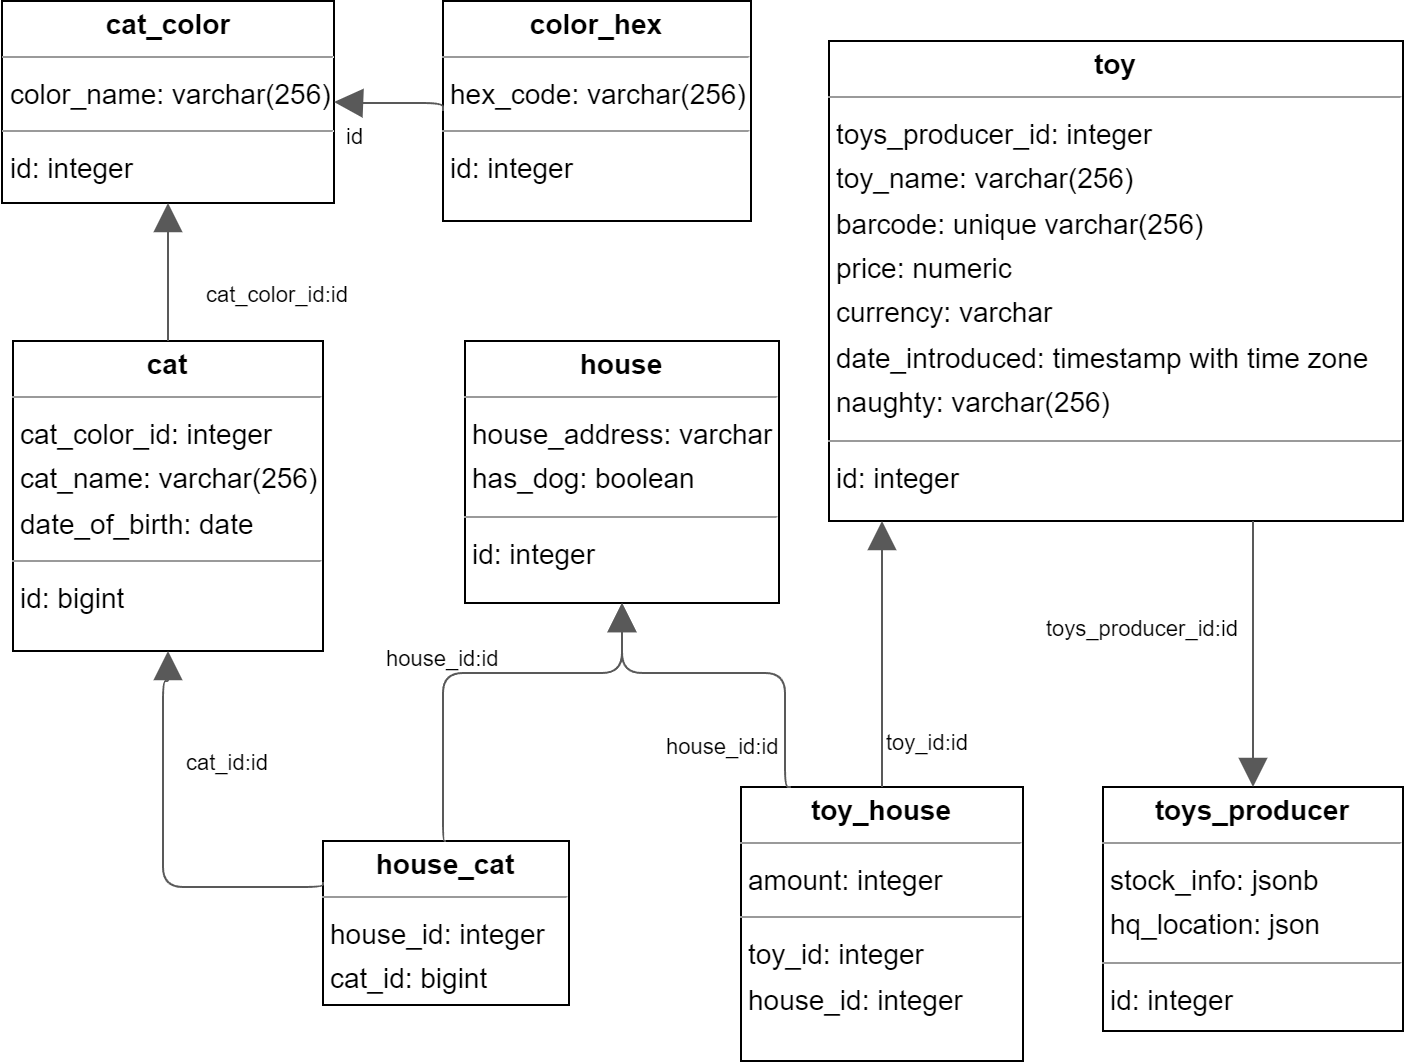
\includegraphics[width=0.9\textwidth]{databaseSchema}
    \caption{Schema of benchmark database}
\end{figure}

\section{Cat Entity}
The \texttt{cat} entity instances represent individual cats which we want to
monitor. Each has a~unique identifier, name and date of birth, all of which are
nullable except for the identifier. This entity aims to represent the basic
database table and to verify the correct handling of the data type from
Postgres, as JavaScript Date time represents a~moment, including time
\cite{JavaScript-Date-MDN}. In contrast, the database entry would only contain
the date \cite{Date/TimeTypes_Postgres}. Additionally, the \texttt{cat} entity
uses big integer data type, and handling numbers beyond the standard range
allocated in JavaScript is tested. The \texttt{cat colour} and \texttt{colour
hex code} are two entities that represent the cat colour by its name and by its
hex code. The entities are intentionally split in this way to use identifying
relation~\cite{Karwin_2010} - the primary key of the hex colour entity is also a
foreign key referencing the id of the cat colour entity.

\section{House and Toy House Entities}
The \texttt{house} entity represents domiciles where the cats spend time at
their behest. The relation must account for ambitious cats using several houses
as their homes. The main aim is to test the difficulty of implementing and using
simple many-to-many relations. The only attribute that provides new data type or
behaviour is the simple \verb|has_dog| attribute, specified as a~Boolean. It is
one of several attributes that test the frameworks' ability to correctly type
and convert the data recovered from the database.

The houses can be equipped with many toys for the cats to use. The relation
between houses and toys is modelled through a~decomposition table which contains
attributes representing the number of the same toy in the house. While the
primary keys are the identifiers of the house and toy, the decomposition with
the amount, rather than several records with an additional identifier, is
designed to test the ability to insert a~record if it does not exist or update
the value referencing its previous state. If more toys are purchased, the owner
of the house does not suddenly throw out all toys they already had; they will
add them to their current pile. This operation is often called \textit{upsert} -
a combination of update and insert, and some database engines, such as
CockroachDB \cite{upsertCockroachDB}, implement it explicitly under this name.
PostgreSQL achieves it using the \texttt{ON CONFLICT} statement in
\texttt{INSERT} query \cite{INSERT_postgres_2023}. It also tests the handling of
composite primary keys, a~standard paradigm in many databases.

\section{Toy and Toys Producer Entity}
The \texttt{toy} entity purpose in testing is in numeric data type used in
\texttt{price} attribute and usage of additional column attributes such as
\texttt{CHECK} constraints or \texttt{DEFAULT} values in the column
\cite{Constraints_Postgres_2023}. Column \texttt{naughty} is focused on commonly
problematic strings in software development, such as special Unicode characters,
emojis and other issues that could come up in handling data from the database,
especially if the encoding is not correctly handled. Toys producers host the
JSON columns to test if it is possible to use advanced JSON traversal and query
operators provided in PostgreSQL \cite{postgres-json} (and their equivalents in
other database management systems).
